\documentclass[aps,prmaterials,reprint,amsmath,amssymb,superscriptaddress]{revtex4-2}
\usepackage{siunitx}
\sisetup{range-phrase = --, range-units = single}
\DeclareSIUnit{\rydberg}{Ry}
\DeclareSIUnit{\atomicunits}{a.u.}
%\usepackage{overpic}
\usepackage{graphicx}% Include figure files
\usepackage{graphicx}
\usepackage[abs]{overpic}
%\usepackage{caption}
\usepackage{tikz} 
\usetikzlibrary{calc}
\usepackage{amsmath}
\usepackage{dcolumn}% Align table columns on decimal point
\usepackage{bm}
\usepackage[colorlinks, linkcolor=blue, citecolor=blue, urlcolor=blue]{hyperref}
\usepackage[utf8]{inputenc}
\usepackage[T1]{fontenc}
\usepackage{mathptmx}
\usepackage{etoolbox}
\usepackage{comment}
\usepackage{subcaption}
\usepackage{booktabs}
\usepackage{float}
\usepackage{changepage}
\usepackage{xcolor}
\usepackage{float}
\usepackage{bm}
\newcommand{\DB}{$\Delta\epsilon$}
\newcommand{\DE}{$\Delta$E$_g$}
\makeatletter
\def\@email#1#2{%
 \endgroup
 \patchcmd{\titleblock@produce}
  {\frontmatter@RRAPformat}
  {\frontmatter@RRAPformat{\produce@RRAP{*#1\href{mailto:#2}{#2}}}\frontmatter@RRAPformat}
  {}{}
}%
\makeatother
\begin{document}

\title[III--V alloy electron mobility]{Calculating electron mobility for III--V alloys (In$_{x}$Ga$_{1-x}$)As and In(As$_{1-x}$Sb$_x$).}
\author{Angus Gentles}
\email{angus@kbgentles.org.uk}
\affiliation{ams-OSRAM AG, Tobelbader Str. 30, 8141 Premst{\"a}tten, Austria}
\affiliation{Institute for Microelectronics, TU Wien, Gusshausstrasse 27-29, 1040 Wien, Austria}

\author{Dominic Waldh{\"o}r}
\email{waldhoer@iue.tuwien.ac.at}
\affiliation{Institute for Microelectronics, TU Wien, Gusshausstrasse 27-29, 1040 Wien, Austria}

\author{Mohammad Dehghani}
\thanks{\href{https://orcid.org/0000-0003-4756-0446}{ORCID: 0000-0003-4756-0446}}
\affiliation{Institute for Microelectronics, TU Wien, Gusshausstrasse 27-29, 1040 Wien, Austria}
\affiliation{Christian Doppler Laboratory for Single-Defect Spectroscopy at the
    Institute for Microelectronics, TU Wien, Vienna, Austria}

\author{Pedram Khakbaz}
\affiliation{Institute for Microelectronics, TU Wien, Gusshausstrasse 27-29, 1040 Wien, Austria}
\affiliation{Christian Doppler Laboratory for Single-Defect Spectroscopy at the
    Institute for Microelectronics, TU Wien, Vienna, Austria}
\author{Rainer Minixhofer}
\affiliation{ams-OSRAM AG, Tobelbader Str. 30, 8141 Premst{\"a}tten, Austria}

\author{Michael Waltl}
\affiliation{Institute for Microelectronics, TU Wien, Gusshausstrasse 27-29, 1040 Wien, Austria}

\date{\today}

\begin{abstract}
We present a first-principles scheme for the electron mobility of direct-gap semiconductor
alloys and apply it to (In$_x$Ga$_{1-x}$)As and In(As$_{1-x}$Sb$_x$). A virtual crystal is
corrected by Hubbard $U$ parameters fitted to supercell effective band structures under an
experimental effective-mass constraint, and the alloy scattering potential is computed
directly rather than estimated from electronegativity differences. Both channels enter the
iterative solution of the Boltzmann transport equation. The computed coupling elements are
three to four times larger than previous estimates and vary strongly with wavevector, which
constant-potential models cannot capture. In In(AsSb), alloy scattering alone reproduces
the measured mobility below \SI{150}{\kelvin}.
\end{abstract}

\maketitle

\section{Introduction}

The performance of a photodetector rests on intrinsic material properties: the band gap and absorber--substrate band offsets, which set carrier generation and confinement\cite{Hao2023}, and the electron mobility, which governs how efficiently the generated carriers are transported to and collected at the contacts\cite{intro_efficienty_Pecunia2019}. Within the (InGa)(AsSb) family, In(As$_{1-x}$Sb$_x$) reaches the smallest gaps of any III--V alloy, with a minimum of \SIrange{0.12}{0.16}{\electronvolt} at \SI{0}{\kelvin} near $x\approx0.6$ depending on the bowing parameter adopted\cite{Cripps2008,Murawski2019}, placing it in the mid-wave infrared. (In$_{0.53}$Ga$_{0.47}$)As occupies the opposite role: it is the most widely used composition in the family\cite{Forrest1980,Zhang2018} because it is lattice matched to InP\cite{Donati2003}, removing the need for strain-relieving buffer layers, and its \SI{0.74}{\electronvolt} room-temperature gap gives a cutoff near \SI{1.7}{\micro\meter} in the short-wave infrared. The two alloys therefore cover complementary spectral ranges, and their small direct gaps and high absorption coefficients make both useful for photodetector arrays\cite{InAsSbPD1_Rogalski2020} and as LED emitters\cite{InGaAsLED1_Yang2020,InAsSbLED1_Mynbaev2017,InGaAsLED2_Grasse2013}. Their composition-dependent transport properties, however, remain poorly characterised from first principles, with the relative contributions of alloy and phonon scattering largely unquantified across the composition range.

The scattering mechanisms that limit electron transport in the III--V binaries were established by semi-empirical solutions of the BTE, first variationally by Ehrenreich\cite{Ehrenreich1957,Ehrenreich1960} and later with Rode's iterative method\cite{Rode1971,Rode1975}. These studies showed that polar optical phonon scattering dominates in GaAs, InAs and InSb near room temperature. Ionized-impurity scattering takes over at low temperature, and acoustic deformation-potential and piezoelectric scattering contribute only weakly. In InSb, whose gap is narrow enough for a significant intrinsic hole population, electron--hole scattering becomes increasingly important at higher temperatures\cite{InSb_mobility_Jung1991}. \textit{Ab initio} transport calculations have since replaced the fitted scattering parameters with electron--phonon matrix elements computed from DFPT. Almost all of this work has concentrated on GaAs\cite{Perturbo1,Liu2017,Ma2018,Brunin2020,Lee2020}, where it established that the iterative solution of the BTE is required for polar materials and that the computed mobility depends strongly on the accuracy of the electron effective mass\cite{Ma2018,Ponce2018}. 

The alloys add a further, elastic scattering channel arising from compositional disorder. The standard treatment reduces the alloy to a primitive cell within the virtual crystal approximation (VCA)\cite{VCA1_Nordheim1931,VCA_alloycorr1}. It then treats the difference between the true and averaged potentials as a perturbation, whose matrix elements between VCA states give the alloy scattering rate\cite{Harrison1976}. Within this framework, the strength of the alloy potential has not been computed but estimated. The options are the band-gap difference, the electron-affinity difference, or, most commonly, the electronegativity difference of the constituents\cite{Phillips1970}. This model has been applied to (InGa)As\cite{Littlejohn1978} and to In(AsSb)\cite{Chin1991,Egan1994}. In each case the mobility was obtained within the relaxation time approximation, using parabolic bands with fitted effective masses. The most complete study of In(AsSb)\cite{Chin1991} found that alloy scattering reduces the room-temperature mobility by at most $\sim$11\%. At low temperature and low doping, however, it becomes the dominant mechanism across most of the composition range. Its importance is therefore strongly regime-dependent, and every estimate of it rests on an empirical potential. First-principles alloy scattering potentials have since been computed for SiGe\cite{MurphyArmando2006,MurphyArmando2008} and GeSn\cite{Sewell2024}, but not for any III--V alloy. The existing picture of alloy transport in In(AsSb) and (InGa)As thus has two weaknesses. The alloy potential is empirical rather than computed, and the phonon-limited part of the calculation uses the approximations that \textit{ab initio} work on the binaries has shown to be unreliable.

Our first two papers approached this problem from two directions, the alloy energetics and the binary mobilities. The first two papers modelled the ternary energetics of (InGa)As, (InGa)Sb, In(AsSb) and Ga(AsSb)\cite{Gentles2024,Gentles2026a}. The first used single $3 \times 3 \times 3$ 54 atom primitive supercells for two mixtures on each alloy, and using a Bayesian process to optimize $U$ parameters for DFT+$U$ calculations on binary crystals\cite{DFTU_Dudarev}, similar to the approach of Yu \textit{et al.}\cite{Yu2020_dftu}, and interpolating these binary $U$ parameters to the alloy mixtures to calculate the alloy bandgaps. The second paper improved and refined this process. The Bayesian optimization was extended to include the bowing itself on small cubic alloy cells directly, and instead of taking a full range of possible $U_p$ values for the anion and cation as the optimization parameters as in the first paper, we instead defined binary-specific iso-$E_g$ contours such that the bandgaps at either end of the alloy, such that the bandgap bowing is a meaningful quantity. Both the bandshape of the binary and the bowing of the alloy bandgaps were combined into a single loss function, then optimized for an compact set of $U$ parameters for each binary. These were interpolated for alloy 64 and 216 atom supercell calculations to produce the effective band structures\cite{EBS_Popescu2010} and the supercell effective masses.

A subsequent study\cite{Dehghani2026} computed the phonon-limited electron mobilities of GaAs, InAs and InSb. The emphasis of that work was on the accuracy of the underlying electronic structure. The DFT$+U$ parameters were optimised against HSE06\cite{hse06} band structures and refined to reproduce the zone-centre phonon frequencies and dielectric constants, and the subsequent DFPT$+U$ calculations and Wannierisation\cite{w901_Mostofi2008,w903_Pizzi2020} were converged with particular attention to the conduction-band curvature. Mobilities were then obtained from the iterative solution of the linearised Boltzmann transport equation in \texttt{PERTURBO}\cite{Perturbo1}. By varying the Hubbard parameters to tune $m^*_\text{e}$ while holding $E_\text{L}$ fixed, the mobility could be computed directly as a function of the effective mass. This showed that $m^*_\text{e}$ is the dominant band-structure parameter controlling phonon-limited transport, and that the conduction band edge must be described accurately before second-order corrections are worth
pursuing.

\section{Mobility Methodology}\label{sec:methodology}

Modelling the electron mobility relies on solving the Boltzmann Transport equation (BTE). The semiclassical BTE for the electron distribution $f_{n\bm{k}}$ is
\begin{equation}
    \frac{\partial f_{n\bm{k}}}{\partial t}
    +\bm{v}_{n\bm{k}}\cdot\nabla_{\bm{r}} f_{n\bm{k}}
    -\frac{e\bm{E}}{\hbar}\cdot\nabla_{\bm{k}} f_{n\bm{k}}
    =\left(\frac{\partial f_{n\bm{k}}}{\partial t}\right)_\text{coll},
    \label{eq:BTE}
\end{equation}
which produces a mobility as 
\begin{equation}
    \mu_{ij} = \frac{e}{n} \int d^{3}k (\rho(\bm{k})) \bm{v}_i \frac{\partial f_{n,\bm{k}}}{\partial E_j},
\end{equation}
where $f$ is the electron distribution function and $n[\bm{k}]$ is the carrier concentration, and $E_j$ is the component of the electric field in the $j$-th direction, and $\rho(\bm{k})$ the density of states at $\bm{k}$. To effectively model this, the distribution function requires an accurate electronic energetic properties, whereas the collision term is dominated by the coupling elements between different $\bm{k}$ points. However, even with the central equation defined, several approximations are necessary to solve it. 

The Self-Energy Relaxation Time Approximation (SERTA) and the Iterative Approach (ITA)\cite{Rode1975} are the standard approximations beyond the highly detailed Monte-Carlo methods. 
The SERTA is the most common approximation for this type of problem\cite{MurphyArmando2008,Chin1991} but has been shown to unreliable results\cite{Ponce2021,Ponce2020,Claes2022,Ma2018}. The ITA, in these papers is significantly more accurate, as it includes in-scattering effects, 

\begin{equation}
\bm{F}_{n\bm{k}}=\tau_{n\bm{k}} \bm{v}_{n\bm{k}}+\tau_{n\bm{k}} \sum_{m\bm{k}^\prime} K_{n\bm{k},m\bm{k}^\prime}\bm{F}_{m,\bm{k}^\prime}\label{eq:ITA1}
\end{equation}

Here $\bm{F}_{n\bm{k}}$ parametrises the linear response of the occupations to the applied field, the $\tau_{n\bm{k}}$ the lifetime of the given state $n,\bm{k}$, and $K_{n\bm{k}}$ the scattering kernel, as defined in Rode\cite{Rode1975}. However, the construction of these objects $F_{n\bm{k}}$, $\tau_{n\bm{k}}$ and $K_{n\bm{k}}$ rely on accurate energetic calculations on the alloys In(AsSb) and (InGa)As. 

The central quantities too accurately modelling the mobilites are the coupling elements $g^\text{el-ph}_{\nu q}(k,k)$ and $g^\text{alloy}(k,k^\prime)$, as well as accurately electronic band structures, especially around the conduction band minimum\cite{Dehghani2026}. Our previous work studied the mobility of the binaries InAs, GaAs and InSb, and found that above very low temperatures, the dominant scattering mechanism was the electron-phonon (e-ph) scattering. The some papers indicate that this should be the case for the alloys too\cite{Chin1991,Rode1983}. However, the approximations for $g^\text{alloy}$ in older papers are taken from less upto date methods such as the electronegativity difference\cite{Phillips1970}, rather than a more recent \textit{ab initio} approaches on different materials\cite{MurphyArmando2006,MurphyArmando2008}. Furthermore, our previous paper highlighted the importance of accurate energetic calculations in calculating the phonon-limited mobility, especially the effective mass ($m^*_\text{e}$), which previous papers didn't focus on\cite{Harrison1976,Rode1983,Chin1991}. However, directly using supercell calculations which are required to accurately model the energetics of these alloys\cite{Gentles2026a} are computationally intractable, requiring a full electron--phonon calculation. A tractable alternative is therefore required.

A common treatment is to regard the alloy as a perturbation to an underlying `pristine' crystal\cite{Harrison1976,Sewell2024}. The electron--phonon interaction is evaluated on this pristine crystal, defined here by the Virtual Crystal Approximation (VCA), while the alloy disorder enters through matrix elements of the residual potential between VCA eigenstates, $\langle\psi_\text{VCA}(n,\bm{k})|\Delta V_\text{alloy}| \psi_\text{VCA}(m,\bm{k}^\prime)\rangle$, evaluated in the first Born approximation.This restores a primitive-cell description of the alloy and makes the transport calculation tractable, but at the cost of an electronic structure that is only as good as the mean field it is built on. In particular, the VCA does not reproduce the conduction-band curvature obtained from supercell calculations, and the resulting error in $m^*_\text{e}$ propagates directly into both scattering channels. Our approach is therefore to retain the supercell energetics as a target rather than as the transport calculation itself: we fit the VCA band structure to the effective band structure of the supercell using Hubbard $U$ parameters as the fitting degrees of freedom. 

\section{Virtual Crystal Approximation and the Hubbard Correction}\label{sec:VCA}

The virtual crystal approximation (VCA) approximates the alloy as a perfect crystal, where the potentials of each lattice are linearly interpolated. In the case of (A$_x$B$_{1-x}$)C, the potential is given by $V_\text{VCA}=x V_\text{A}+(1-x)V_\text{B}$. Usually the VCA tends to be avoided for many properties such as the bandgap or the effective mass, as it very often shows a perfectly linear variation. Indeed, in the previous paper of this group the VCA was compared to a supercell technique, and it showed a perfectly linear variation of the bandgap, inconsistently with both the supercell technique and experimental data\cite{Gentles2026a}. 
Although the bandgap is not itself a target quantity, mobility calculations require a finite gap, and the underestimation of gaps by (semi-)local functionals\cite{Perdew2009} also distorts the band shape; this is critical for InAs, InSb and GaSb, which LDA and PBE predict to be gapless semimetals\cite{derivativedis_Perdew1983}.


The effective mass is a critical input to the mobility\cite{Dehghani2025}, yet the VCA necessarily interpolates $m^*_\text{e}$ linearly between the constituent binaries, irrespective of how well the underlying functional describes them, in disagreement with the experimental data collated in Fig.~1 of the Supplemental Material. Since the VCA phonon dispersion instead reproduces the supercell result reasonably well \cite{MurphyArmando2008}, the deficiency to be addressed is electronic: we require a correction to the VCA band structure that is compact, self-consistent, and compatible with the \texttt{quantum ESPRESSO} toolchain used to extract phonon-limited mobilities.

A compact correction of this kind is available in the Hubbard-corrected DFT$+U$ framework\cite{DFTU_Dudarev}. In our previous study\cite{Gentles2026a,Angus_syspad} we used DFT$+U$ to compute effective band structures for supercells of (In$_x$Ga$_{1-x}$)As, (In$_x$Ga$_{1-x}$)Sb, In(As$_{1-x}$Sb$_x$) and Ga(As$_{1-x}$Sb$_x$); these serve here as reference band structures against which the VCA can be fitted, using $U$ as the degree of freedom. We therefore adjust the VCA band structure within a VCA+$U$ framework to reproduce the experimental effective mass near the conduction band minimum and the reference effective band structure away from it.

The Dudarev formulation of DFT$+U$, a Hubbard like energy correction term is added to the DFT energy of the form

\begin{equation}
	E_{\mathrm{Hub},X}
	= \frac{U_{\mathrm{eff},X}}{2}
	\sum_{\sigma}
	\left[
	\mathrm{Tr}\!\left(\bm{n}_{\sigma,X}\right)
	- \mathrm{Tr}\!\left(\bm{n}_{\sigma,X}^{2}\right)
	\right]
	\label{eq:DFT_U_energy}
\end{equation}

where $U_{\text{eff},X}$ is the effective Hubbard parameter for the electron manifold $X$ and $\bm{n}_{\sigma,X}$ the corresponding occupation matrix for spin $\sigma$. The term penalises fractional occupations, increasing the localisation of the manifold, and thereby provides a compact, orbital-resolved perturbation of the electron density; see our previous paper\cite{Gentles2026a} for the full formalism. Following that work, we correct only the valence $p$ manifolds and write $U$ for $U_\text{eff}$ and $U_A$ for the parameter on species $A$, giving the two-dimensional space $\bm{U}=(U_A,U_B)$ for a ternary with cation $A$ and anion $B$. The rationale is given there in full: the $p$ states dominate the valence bands and, through hybridisation with the cation $s$ states, also the conduction bands, whereas correcting the $s$ manifold directly mainly shifts the $\Gamma$-valley gap and can degrade $m^*_\text{e}$. Restricting the correction to $p$ additionally improves the phonon dispersions relative to PBE\cite{Dehghani2026,Gentles2026a}, which matters here because the same parameters enter the DFPT+$U$ calculation of the electron--phonon coupling. The task is therefore reduced to locating a single point in the two-dimensional space $\bm{U}=(U_A,U_B)$ for each composition.

\begin{figure}[h!]
    \centering
    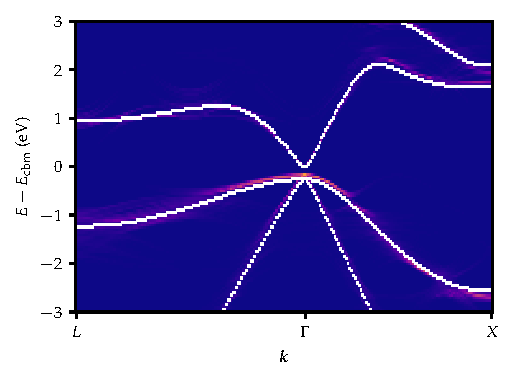
\includegraphics{Figures/In1.0Ga0.0As0.5Sb0.5_EBS.pdf}
    \caption{The EBS of InAs$_{0.5}$Sb$_{0.5}$ overlaid with the optimum VCA mask, with $(U^\text{In}_{5p},U^\text{As$_{0.5}$Sb$_{0.5}$}_{5p})$. Summing through the white tiles gives the loss function.}
    \label{fig:fit_example}
\end{figure}

The reference EBSs are taken directly from our previous work\cite{Gentles2026a}: for each composition, ten SQS supercells generated with \texttt{SQSgenerator}\cite{sqsgen} were computed with DFT$+U$ and unfolded onto the primitive-cell Brillouin zone. Beyond providing a reference dispersion, the unfolding supplies a natural weighting function for the fit. Each supercell eigenstate $|\Psi_{m\bm{K}}\rangle$ at a supercell wavevector $\bm{K}$ is projected onto the primitive-cell Bloch states $|\varphi_{n\bm{k}}\rangle$ with $\bm{K}=\bm{k}+\bm{G}$, giving the spectral function
\begin{equation}
    A(\bm{k},E)=\sum_{m,n}\big|\langle\Psi_{m\bm{K}}|\varphi_{n\bm{k}}\rangle\big|^{2}\,
    \delta(\varepsilon_{m\bm{K}}-E),
\end{equation}
which measures the likelihood of an eigenvalue of the alloy lying at energy $E$ and wavevector $\bm{k}$. We discretise $A$ on an energy grid of \SI{0.05}{\electronvolt} and sum the ten configurations, with each EBS zeroed to its conduction band minimum, to obtain the discrete spectral weight $s(\bm{k},\varepsilon)$. A candidate VCA+$U$ band structure is then scored by summing the weight of the cells its eigenvalues fall into,
\begin{equation}
    \zeta_0 = \sum_{i,j} s(\bm{k}_i,\varepsilon_{j}(\bm{U})),
    \label{eq:loss_zeta0}
\end{equation}
where $i$ runs over the $\bm{k}$-points of the high-symmetry path and $j$ over the VCA$+U$ bands, both zeroed to the conduction band minimum. Figure~\ref{fig:fit_example} shows the combined EBS of InAs$_{0.5}$Sb$_{0.5}$ overlaid with the optimal VCA$+U$ mask. Maximising $\zeta_0$ alone is nonetheless inadequate, for two reasons. First, the weighting is uniform: every $\bm{k}$-point on the path contributes equally, so the fit is driven as much by regions far outside the energy window relevant to transport as by the states that carry the current. Second, the resolution is insufficient: the $\bm{k}$-point spacing along the path is too coarse for the sum to constrain the band curvature at $\Gamma$, and hence the effective mass. We address the weighting by modifying $\zeta_0$ itself, and the resolution by restricting the parameter space it is evaluated on.

The weighting is corrected by multiplying the summand by a Gaussian envelope centred on the conduction band minimum, of standard deviation $E_\text{MW}$, so that the fit is dominated by the transport-relevant states. We set $E_\text{MW}=\SI{1.0}{\electronvolt}$, the energy range over which conduction states contribute appreciably to the transport integrals at the temperatures considered here. The envelope remains broad enough to retain finite weight at the valence band edge, so a VCA$+U$ band structure whose gap is badly in error places its valence bands where the EBS carries no spectral weight and is penalised accordingly.

The resolution cannot be corrected the same way, since the envelope changes which parts of the dispersion are weighted, not how finely the curvature at the band edge is resolved. We therefore impose the effective mass as a hard constraint on the search rather than fitting it. Where our previous work constrained $\bm{U}$ to an iso-$E_g$ contour\cite{Gentles2026a}, here we constrain it to an iso-$m^*_\text{e}$ contour, retaining only those $\bm{U}$ whose $\Gamma$-valley mass agrees with experiment to within a tolerance $\Delta m^*$. For In(AsSb) and (InGa)As, experimental masses are available across the composition range to two significant figures (collated in the Supplemental Material), which makes this constraint well defined. Combining the two corrections gives the objective
\begin{equation}
    \zeta = \sum_{i,j} s(\bm{k}_i,\varepsilon_j)\,
    \exp\!\left[-\frac{(\varepsilon_j-E_\text{cbm})^2}{2E_\text{MW}^2}\right]
    \bigg|_{\,|m^*_\text{e}(\bm{U})-m^*_{e,\text{exp}}|<\Delta m^*},
    \label{eq:loss_function}
\end{equation}
which is maximised over $\bm{U}$ subject to that constraint.

\begin{figure} 
    \centering 
    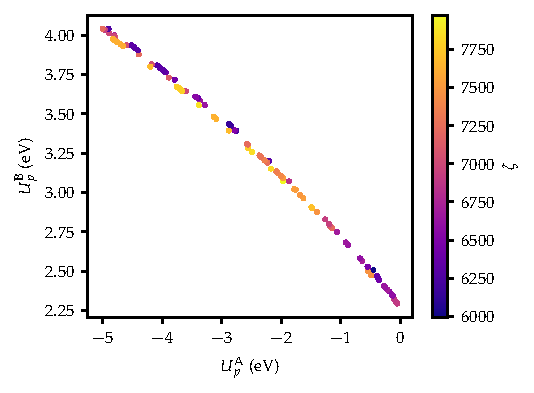
\includegraphics{Figures/weights_vs_Us.pdf} 
    \caption{The $\bm{U}|_{m^*=m^*_\text{exp}}$ isobar points coloured by their $\zeta$ function values for In(As$_{0.5}$Sb$_0.5$).} 
    \label{fig:weights} 
\end{figure} 

To sample $\zeta$ over the admissible region of $\bm{U}$, an initial grid of $\bm{U}=(U^\text{A}_p,U^\text{B}_p)$ pairs was generated, where A and B denote the cation and anion species respectively, spanning $U^\text{A}_p \in [-5,5]$~eV and $U^\text{B}_p \in [0,8]$~eV in steps of \SI{0.2}{\electronvolt}. Each pair was passed through a sequence of structural relaxation, SCF, NSCF band-structure and NSCF effective-mass calculations. A spline was fitted to the resulting grid of effective masses and used to locate the iso-$m^*_\text{e}$ contour; further points were then sampled along that contour and the spline updated with them. The objective $\zeta$ of Eq.~\eqref{eq:loss_function} was evaluated at each admissible point, and the maximising $\bm{U}$ taken as the system-representative parameter set; the resulting values for each composition are given in the Supplemental Material. The tolerance corresponds to the two-significant-figure precision of the experimental masses; being absolute rather than relative, it constrains the light-mass, Sb-rich compositions less tightly than the As-rich ones. 

This provides a scheme for generating VCA$+U$ parameters for each alloy composition, which serve as the starting point for the transport calculation proper: the same parameters enter the DFPT$+U$ calculation of the phonon dispersions and electron--phonon matrix elements $g^\text{el-ph}_{\nu\bm{q}}(\bm{k},\bm{k}+\bm{q})$, while the VCA eigenstates provide the basis in which the alloy matrix elements $g^\text{al}(\bm{k},\bm{k}^\prime)$ are evaluated.The construction of the alloy scattering is described in Sec.~\ref{sec:alloy_scattering} and the electron--phonon scattering in Sec.~\ref{sec:eph_scattering}, with their incorporation into the ITA given in Sec.~\ref{sec:implementation}.

\section{Alloy Scattering}\label{sec:alloy_scattering}

Alloy scattering originates from the difference between the averaged potential of the virtual crystal and the true potential of the atoms occupying the lattice in the real alloy. This residual potential is static, with no phonons involved to change the energies, so the mechanism is elastic and only the direction of the carrier momentum is altered. The alloys studied here are direct-gap materials with the conduction band minimum at $\Gamma$, and the $L$ valley of the constituent binaries lies at least \SI{0.8}{\electronvolt} higher, whereas the transport window extends only $\sim 8k_\text{B}T \approx \SI{0.2}{\electronvolt}$ above the band edge at room temperature. Inter-valley scattering can therefore be disregarded across the temperature range considered here.

The central quantity of the alloy scattering is the coupling element $g^\text{alloy}(\bm{k},\bm{k}^\prime)$, whose square determines the scattering rate through Fermi's golden rule. Over the past two decades an \textit{ab initio} route to these coupling elements has been developed within the RTA framework for Si$_x$Ge$_{1-x}$\cite{MurphyArmando2006,MurphyArmando2008} and Ge$_x$Sn$_{1-x}$\cite{Sewell2025}. The real element (Ga, In, As or Sb) is treated as a defect substituted into a VCA supercell, and the resulting change in the potential provides the perturbation. The formalism rests on several assumptions. First, the scattering sites interact weakly with the electrons, so that each site can be treated independently. Second, the alloy is completely random, which reduces the composition dependence to a simple factor of $x(1-x)$ rather than a dependence on the short-range order parameter\cite{Harrison1976} used in our previous work\cite{Gentles2026a}. Third, the averaged crystal does not itself scatter, so that only the substituted atoms contribute. To these we add a fourth. Murphy-Armando and Fahy evaluate the matrix element between a VCA state and the supercell wavefunction, which retains the distortion of the scattering state by the substituted atom; we instead take both states to be unperturbed VCA eigenstates, which is the first Born approximation. This gives the alloy coupling element as

\begin{equation}
    |g^\text{alloy}(\bm{k},\bm{k}^\prime)|^2 = x(1-x) \frac{1}{\Omega_0^2} | \langle \psi^\text{VCA}_{\bm{k}^\prime} | \Delta V | \psi^\text{VCA}_{\bm{k}} \rangle|^2,\label{eq:alloy_scattering}
\end{equation}

where $\psi^\text{VCA}_{n\bm{k}}$ is a VCA eigenstate normalised to unit mean density, $V^{-1}\!\int_V|\psi|^2\,d^3R = 1$, and $\Omega_0$ is the volume per alloying site. For a zincblende alloy mixed on a single sublattice $\Omega_0$ coincides with the primitive-cell volume, $\Omega_0 = a_0^3/4$ in terms of the conventional cubic lattice constant.

Their formalism further assumes a single scattering rate per valley, independent of $\bm{k}$. We are aware of no published assessment of how good this approximation is in a direct-gap III--V alloy, and we therefore retain the full $(\bm{k},\bm{k}^\prime)$ dependence of the matrix element rather than reducing it to a constant.

For the perturbing potential, Murphy-Armando and Fahy write
\begin{equation}
    \Delta V = N (V_\text{A}-V_\text{B})
    \label{eq:deltaV_MA}
\end{equation}
for an alloy (A$_x$B$_{1-x}$)C or C(A$_{1-x}$B$_x$), where $N$ is the number of alloying sites in the supercell\cite{MurphyArmando2008}. They then transform from the primitive-cell VCA wavefunctions to the supercell wavefunctions, a step that relies on the degeneracy of the $X$ and $L$ valleys and has no counterpart at $\Gamma$; this is what forces the first Born approximation introduced above. In the present work the site counting is carried entirely by the $x(1-x)$ and $\Omega_0^{-2}$ factors of Eq.~\eqref{eq:alloy_scattering}, so the perturbation is simply the difference of the two constituent potentials, $\Delta V = V_\text{A}-V_\text{B}$, evaluated at the VCA equilibrium lattice constant.

Instead we evaluate these matrix elements directly. The VCA eigenstates are transferred to a real-space grid of $80\times 80\times 80$ points for (In$_x$Ga$_{1-x}$)As and $90\times 90\times 90$ for In(As$_{1-x}$Sb$_x$), and the supercell potentials are generated on grids of $240\times 240\times 240$ and $270\times 270\times 270$ points respectively, three times denser in each direction so that every supercell grid point maps onto a primitive-cell grid point under the supercell transformation. The perturbation $\Delta V(\bm{R})$ is obtained as the difference between the self-consistent potentials of two otherwise identical supercells, one with species A and one with species B at the substituted site. The matrix element is then
\begin{equation}
    M_{mn}(\bm{k},\bm{k}^\prime)= \frac{1}{\Omega_0}
    \int_{V_\text{SC}} d^3R\; \psi^{*}_{m\bm{k}^\prime}(\bm{R})\,
    \Delta V(\bm{R})\,\psi_{n\bm{k}}(\bm{R}),
    \label{eq:matrix_element}
\end{equation}
with the integral taken over the supercell volume $V_\text{SC}$, so that the alloy coupling element of Eq.~\eqref{eq:alloy_scattering} is $|g^\text{alloy}(\bm{k},\bm{k}^\prime)|^2 = x(1-x)\,|M_{mn}(\bm{k},\bm{k}^\prime)|^2$.

The matrix element of Eq.~\eqref{eq:matrix_element} contains the Bloch phase factor $e^{i(\bm{k}-\bm{k}^\prime)\cdot\bm{R}}$ multiplying the overlap of the cell-periodic parts. Representing that phase exactly requires the two wavevectors to be commensurate with the supercell, which for the small $|\bm{k}|$ relevant to transport in these light-mass bands would demand prohibitively large cells. We therefore omit the phase factor and retain only the cell-periodic overlap. This is justified by the short range of $\Delta V$, which decays within a few bond lengths of the substituted site: over the region in which the integrand carries appreciable weight, $(\bm{k}-\bm{k}^\prime)\cdot\bm{R}\ll 1$ for every pair of wavevectors in the transport window. The arbitrary relative phase between the two VCA eigenstates is removed separately, by aligning them before the integral is evaluated.

The VCA$+U$ parameters obtained in Sec.~\ref{sec:VCA} are used for the primitive cell, while the substituted supercells use the Hubbard parameters of the pure binaries from our previous work\cite{Gentles2026a}. The supercells are cubic and contain 216 atoms, corresponding to 108 primitive cells, and the primitive-cell eigenstates are replicated onto the supercell grid according to the supercell transformation matrix.

\begin{figure}[h]
    \centering
    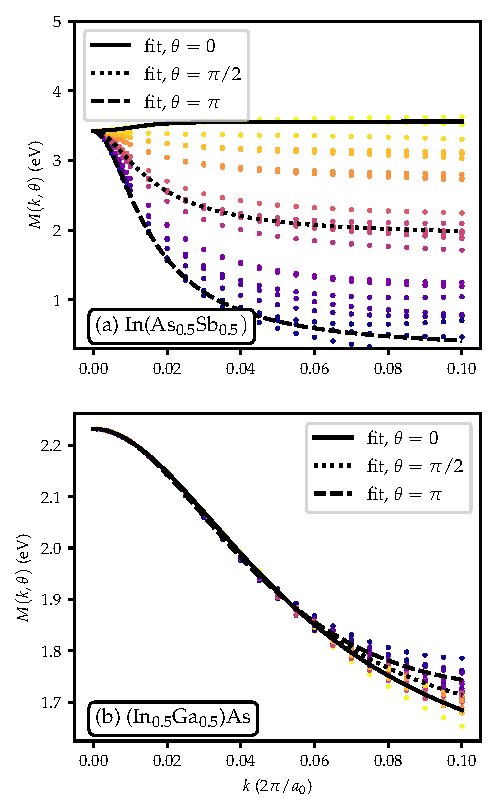
\includegraphics{Figures/coupling_elements.pdf}
    \caption{Alloy coupling elements $M(k,\theta)$ for (a) In(As$_{0.5}$Sb$_{0.5}$), mixed on the anion sublattice, and (b) (In$_{0.5}$Ga$_{0.5}$)As, mixed on the cation sublattice, plotted against $|\bm{k}|$ in units of $2\pi/a_0$. The colour of each point encodes $\cos\theta$, where $\theta$ is the angle between $\bm{k}$ and $\bm{k}^\prime$. Black lines show the fitted function of Eq.~\eqref{eq:fit} evaluated at $\theta=0$ (solid), $\pi/2$ (dotted) and $\pi$ (dashed). The anion-mixed alloy shows both a larger coupling and a considerably stronger angular dependence than the cation-mixed one.}
    \label{fig:coupling_elements}
\end{figure}

The computed $M(\bm{k},\bm{k}^\prime)$ is reparameterised in spherical coordinates. The azimuthal angle $\phi$ is omitted because the conduction band is isotropic about $\Gamma$ to a good approximation across the transport window, leaving a dependence on $k=|\bm{k}|$ and on $\cos\theta = \bm{k}\cdot\bm{k}^\prime/kk^\prime$ alone, with elasticity fixing $|\bm{k}^\prime|=|\bm{k}|$. We evaluate $M(k,\theta)$ on 28 spheres of increasing radius, each sampled by 26 $\bm{k}$-points, giving 351 distinct pairs per shell. The results are shown in Fig.~\ref{fig:coupling_elements} for In(As$_{0.5}$Sb$_{0.5}$) and (In$_{0.5}$Ga$_{0.5}$)As. 
The two alloys behave differently. In the anion-mixed In(As$_{0.5}$Sb$_{0.5}$) the coupling at $\theta=0$ rises slightly towards an asymptote while that at $\theta=\pi$ falls to a lower one, whereas in the cation-mixed (In$_{0.5}$Ga$_{0.5}$)As it decreases with $k$ at all angles. The difference originates in the orbital character of the conduction band and in which sublattice carries the perturbation. At $\Gamma$ the conduction band minimum is of pure $s$ character, but away from the zone centre it acquires an admixture of $p$ character whose amplitude grows with $|\bm{k}|$ and which is almost entirely anion-derived\cite{Gentles2026a}. Since that $p$ orbital is oriented along $\bm{k}$, the overlap of two such states varies linearly with $\cos\theta$, as assumed in Eq.~\eqref{eq:fit}, whereas the $s$ component contributes no angular dependence. In In(AsSb) the perturbing potential sits on the anion sublattice, where the $p$ amplitude is concentrated, and the matrix element therefore acquires a pronounced angular dependence. In (InGa)As it sits on the cation sublattice, where the conduction states remain essentially $s$-like, and the coupling is correspondingly isotropic, varying only with $|\bm{k}|$.

These data are fitted to an empirical function,
\begin{equation}
    M(k,\theta) = M_{00} + S(k)\left[\,M_{1} + f(k)\,(1-\cos\theta)\right],
    \label{eq:fit}
\end{equation}
with the switch-on and angular-strength functions
\begin{equation}
    S(k) = 1 - e^{-(k/k_\text{t})^{m}},
    \qquad
    f(k) = \frac{A}{1+(k/k_0)^{n}} + C.
    \label{eq:fit_components}
\end{equation}
Here $M_{00}$ is the long-wavelength limit of the coupling, approached as $k\to0$ where $S(k)\to0$ and the scattering becomes isotropic. The switch-on function $S(k)$ turns on both the isotropic deviation $M_1$ and the angular dependence over the characteristic scale $k_\text{t}$, with $m$ setting how abruptly, while $f(k)$ sets the strength of the $(1-\cos\theta)$ anisotropy, decaying from $A+C$ at small $k$ to $C$ at large $k$ over the scale $k_0$. The fit is performed over all $9828$ computed matrix elements simultaneously, and the resulting parameters for each composition are given in the Supplemental Material.

\textcolor{red}{The predicted coupling elements are three to four times larger than those of earlier studies~\cite{Littlejohn1978,Chin1991}, corresponding to roughly an order of magnitude in the scattering rate. Those studies estimate the alloy scattering potential from the dielectric electronegativity theory of Phillips~\cite{Phillips1970}, in which the disorder is identified with the fluctuation in the heteropolar (ionic) part of the crystal energy.}
For a binary A$^\text{III}$B$^\text{V}$ compound this energy is
\begin{equation}
    C_{AB} = \frac{b\,e^{2}}{4\pi\epsilon_{0}}
      \left( \frac{Z_{A}}{r_{A}} - \frac{Z_{B}}{r_{B}} \right) e^{-k_{s} R},
\end{equation}
\textcolor{red}{with $Z_A=3$ and $Z_B=5$ the valence numbers, $r_A$ and $r_B$ the covalent radii, $R=\tfrac{1}{2}(r_A+r_B)$, and $k_s$ the Thomas--Fermi screening wavenumber; the empirical factor $b$ corrects for the overestimate of screening by the Thomas--Fermi approximation at small interatomic separations. The alloy scattering potential is the difference between the two constituent binaries, $\Delta U = |C_{\mathrm{InAs}}-C_{\mathrm{InSb}}|$, in which the common cation contribution cancels. Following Harrison and Hauser~\cite{Harrison1976}, this potential is taken as a constant square well filling each anion cell, which gives a matrix element with no $\bm{k}$ dependence, and yields $\Delta U \approx 0.80$~eV for InAs$_{1-x}$Sb$_{x}$ at $x=0.5$~\cite{Littlejohn1978}.}

\textcolor{red}{Two difficulties attend this estimate. First, it rests on a predominantly ionic picture of the bonding, with the bonding charge treated as localised at the bond centre and the disorder represented by a square well, so it takes no account of the shape of either the true potential or the scattering states. Second, it is not the only such estimate available: the same quantity obtained from the electron affinity diffrence or the band gap difference gives 0.31 and 0.18~eV respectively for InAs$_{1-x}$Sb$_{x}$, a spread of more than a factor of four, and the ordering of the three estimates varies from alloy to alloy~\cite{Littlejohn1978}. Littlejohn \textit{et al.} note that there are no firm theoretical or experimental grounds for preferring one of them. A first-principles evaluation of $\Delta V$ supplies the independent determination that these models could not provide for themselves.}

\section{Electron-Phonon Coupling}\label{sec:eph_scattering}

Like the alloy scattering, the electron--phonon scattering depends on the electronic band structure, but it additionally requires an accurate phonon dispersion and the coupling between the two, which enter through the matrix element $g^\text{eph}_{\bm{q}\nu}(\bm{k},\bm{k}+\bm{q})$. Evaluating this quantity directly in a disordered supercell is prohibitively expensive, since even the phonon dispersion of a 216-atom cell is a substantial calculation and the electron--phonon coupling requires the linear response to every atomic displacement in that cell. We therefore follow the conventional approach of computing the lattice dynamics within the VCA and Wannier interpolating the resulting coupling elements\cite{Marzari1997,Giustino2007,Giustino2017}, verifying the VCA phonon density of states against that of the 64-atom supercells. The toolchain is otherwise that of our previous study of phonon-limited mobility in the binary crystals\cite{Dehghani2026}.
This section sets out the phonon calculations, their validation against the supercells, and the treatment of the long-range polar coupling, which requires particular care in these narrow-gap alloys.

\begin{figure}[h] 
    \centering 
    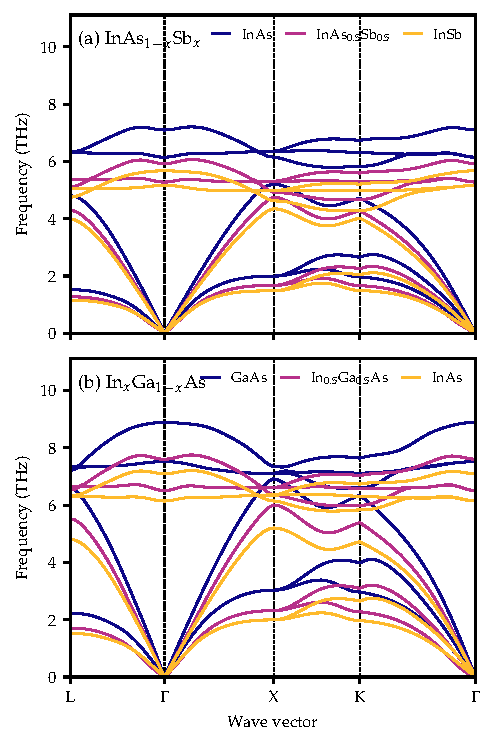
\includegraphics{Figures/all.freq.offset.pdf} 
    \caption{Phonon dispersions of (a) InAs, In(As$_{0.5}$Sb$_{0.5}$) and InSb, and (b) GaAs, (In$_{0.5}$Ga$_{0.5}$)As and InAs, calculated with DFPT$+U$ within the VCA. No imaginary frequencies occur anywhere in the Brillouin zone, confirming the dynamical stability of the virtual crystals. The alloy branches do not lie midway between those of the constituent binaries, so the VCA dispersion is not a linear interpolation of the binary dispersions despite the linear interpolation of the potentials.}
    \label{fig:phonons} 
\end{figure}

\begin{figure}[h] 
    \centering 
    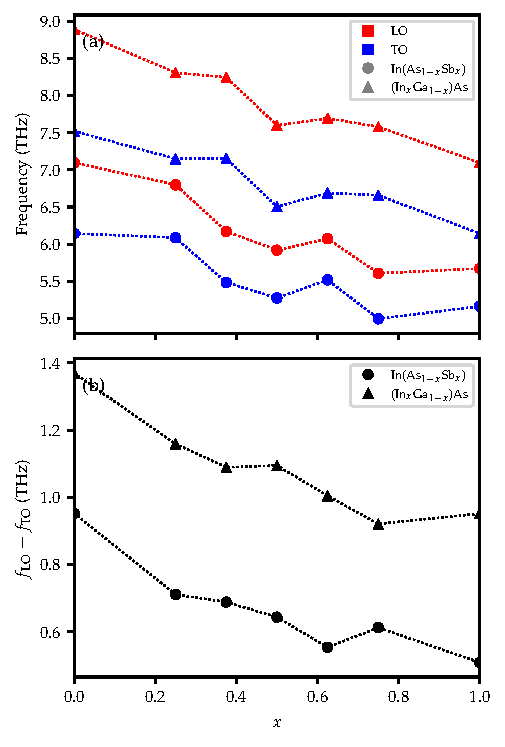
\includegraphics{Figures/all.LO-TO.combined.offset.pdf} 
    \caption{(a) Zone-centre transverse-optical (TO) and longitudinal-optical (LO) phonon frequencies of In(As$_{1-x}$Sb$_x$) and (In$_x$Ga$_{1-x}$)As obtained from DFPT$+U$ within the VCA. (b) The corresponding LO--TO splitting. The splitting in (In$_x$Ga$_{1-x}$)As decreases monotonically and close to linearly across the composition range, whereas In(As$_{1-x}$Sb$_x$) exhibits a pronounced minimum near $x\approx0.62$, at which the splitting falls below the value of either binary endpoint. Dotted lines are guides to the eye.}
    \label{fig:TO_LO} 
\end{figure}


The phonon calculations for each composition use the $U$ parameters obtained in Sec.~\ref{sec:VCA}. The DFPT$+U$ procedure follows that of our previous work\cite{Gentles2026a}, with a self-consistent-field $\bm{k}$-point grid of $16\times16\times16$ and a DFPT$+U$ $\bm{q}$-point grid of $8\times8\times8$ with a $1 \times 1 \times 1$ grid offset, both generated within the Monkhorst--Pack scheme\cite{monkhorstpack_Monkhorst1976}. Each virtual atom was assigned the composition-weighted average of the masses of the two species it represents. The phonon dispersions of GaAs, (In$_{0.5}$Ga$_{0.5}$)As, InAs, In(As$_{0.5}$Sb$_{0.5}$) and InSb are shown in Fig.~\ref{fig:phonons}, and the zone-centre TO and LO frequencies and their splitting in Fig.~\ref{fig:TO_LO}.
The two alloys show different trends in the zone-centre optical modes. In (In$_x$Ga$_{1-x}$)As both the TO and LO frequencies soften steadily with increasing In content, and the LO--TO splitting decreases monotonically and close to linearly across the composition range. In In(As$_{1-x}$Sb$_x$) the splitting instead passes through a minimum near $x\approx0.62$, where it falls below the value obtained for either binary endpoint. Since the splitting is set by the Born effective charges and the electronic dielectric constant, both of which vary with composition, this non-monotonic behaviour is not captured by a simple interpolation between the binaries.


\begin{figure}
    \centering 
    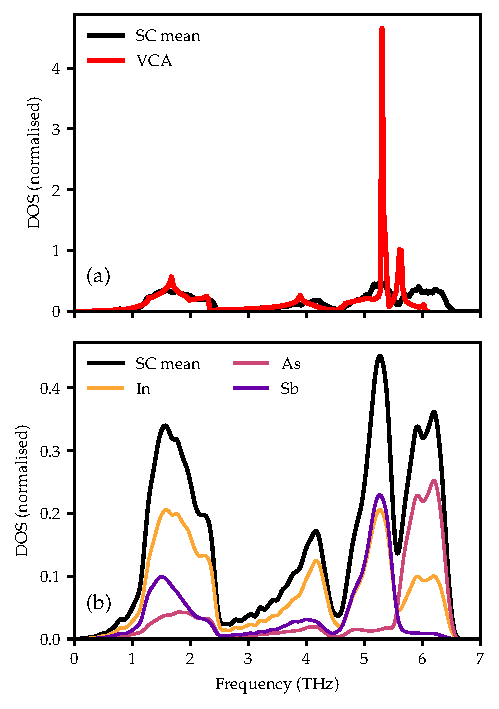
\includegraphics{Figures/In1.0Ga0.0As0.5Sb0.5_dos.both.pdf} 
    \caption{Phonon density of states of In(As$_{0.5}$Sb$_{0.5}$). (a) Configuration-averaged density of states of the six 64-atom supercells (black), computed by the finite displacement method, compared with that of the VCA$+U$ primitive cell (red). (b) The same supercell density of states resolved by species. All curves are normalised to unit area in (a), and in (b) the projections are normalised by the area of the supercell total so that their relative weights are preserved.}
    \label{fig:VCA_vs_SC_phonon} 
\end{figure}

The resulting VCA phonon densities of states were compared with those of the In(As$_{0.5}$Sb$_{0.5}$) supercell configurations of our previous work\cite{Gentles2026a}, for which the force constants were obtained by the finite displacement method as implemented in \texttt{Phonopy}\cite{phonopy1_Togo2023,phononpy2_Togo2023a}. The densities of states of the individual configurations were summed to give a configuration-averaged total, shown in Fig.~\ref{fig:VCA_vs_SC_phonon}. Only the equiatomic composition was treated, both because of the computational cost and because it represents the worst case for the VCA, the configurational disorder being maximal there.

The acoustic region is well reproduced, the VCA and supercell densities of states agreeing in both the positions and the weights of their features below \SI{2.5}{\tera\hertz}. In the optical region the supercell density of states separates into two bands which the VCA does not resolve. Projecting onto the constituent species shows these to be of distinct character: the lower band, centred at \SI{5.22}{\tera\hertz}, involves Sb and In motion, while the upper, centred at \SI{5.97}{\tera\hertz}, involves As and In. This is two-mode behaviour, in which the disordered anion sublattice supports separate InSb-like and InAs-like optical branches. A virtual crystal built from averaged masses and potentials admits only a single optical pair, and reproduces the lower, InSb-like branch.

The consequence for the transport calculation is bounded. The strength of the Fr{\"o}hlich interaction is set by $\epsilon_\infty$, $\epsilon_\text{s}$ and the Born effective charges, which are macroscopic quantities the VCA reproduces, rather than by the distribution of oscillator strength between modes. Placing the whole of that strength on the lower branch raises the phonon occupation $N_\text{LO}$ by \SI{12}{\percent} at \SI{300}{\kelvin} relative to the species-weighted value, corresponding to a \SI{7}{\percent} overestimate of the polar scattering rate; the effect is limited because $\hbar\omega_\text{LO}\lesssim k_\text{B}T$, where the rate depends only weakly on the mode frequency. We note this as a systematic of the virtual-crystal description rather than a source of the discrepancies discussed in Sec.~\ref{sec:results}.

This comparison establishes agreement in the phonon frequencies, but not directly in the electron--phonon matrix elements, which depend additionally on the mode eigenvectors and on the perturbed potentials they generate. A direct test of the couplings would require the supercell electron--phonon calculation that the present approach is designed to avoid. We therefore take the agreement in the acoustic density of states, together with the bounded error in the optical frequencies, as evidence that the VCA$+U$ lattice dynamics provide a usable basis for the transport calculation, following the same reasoning applied to Si$_x$Ge$_{1-x}$ by Murphy-Armando and Fahy\cite{MurphyArmando2008}.

Polar-optical phonon scattering depends on the electronic dielectric constant $\epsilon_\infty$ through the long-range Fr{\"o}hlich interaction\cite{Froehlich1954,Verdi2015,Sjakste2015}, whose coupling matrix element is 
\begin{equation}
    M(q) = -\frac{i}{q} \left[ \frac{e^2 \hbar \omega_{\mathrm{LO}}}
    {2V\epsilon_0} \left( \frac{1}{\epsilon_\infty} - \frac{1}{\epsilon_\text{s}} \right)
    \right]^{1/2},
    \label{eq:frohlich}
\end{equation}
where $V$ is the cell volume and $\epsilon_\text{s}$ the static dielectric constant. This contribution is treated separately by \texttt{Quantum ESPRESSO} in computing the LO mode of a polar semiconductor, and by \texttt{PERTURBO} in interpolating the coupling elements.

This can be split into two parts
\begin{equation}
    M^\text{Fr}(q) = -\frac{i}{q} \left[ \frac{e^2 \hbar }
    {2V\epsilon_0} F_\text{Fr}(\omega_{\mathrm{TO}},\omega_{\mathrm{LO}},\epsilon_\infty)
    \right]^{1/2},
    \label{eq:frohlich1}
\end{equation}

\begin{equation}
    F^\text{Fr}(\omega_{\mathrm{TO}},\omega_{\mathrm{LO}},\epsilon_\infty) =  \frac{\omega_{\mathrm{LO}}^2 -\omega_{\mathrm{TO}}^2}{\epsilon_\infty \omega_\mathrm{LO}},
    \label{eq:frohlich2}
\end{equation}
to split the constants and the material-dependent parameters. Equation~\ref{eq:frohlich2} has also used the Lyddane-Sachs-Teller relation\cite{LDS}. the relation is used to compare the Polar-Optical scattering strength between the computational values and experimental estimates. As was shown earlier, the real alloy phonon DOS shows peaks for both constituent elements, in the case of the alloy A(B$_{1-x}$C$_x$) for the binaries AB and AC. When calculating the experimental estimate to $F^\text{Fr}$, we used a weighted scheme that took account of both the AB and AC branches whilst using a linearly interpolated value of $\epsilon_\infty$ such that 
\begin{equation}
    \begin{split}
    F_\text{exp}^\text{Fr}(x)&= x F^\text{Fr}(\omega^\text{AC}_\text{LO},\omega^\text{AC}_\text{TO},x\epsilon^\text{AC}_\infty+(1-x)\epsilon^\text{AB}_\infty)\\ &+(1-x) F^\text{Fr}(\omega^\text{AB}_\text{LO},\omega^\text{AB}_\text{TO},x\epsilon^\text{AC}_\infty+(1-x)\epsilon^\text{AB}_\infty).  
    \end{split}
    \label{eq:frohlich_exp}
\end{equation}

These quantities, especially the ratio $F_\text{exp}^\text{Fr}/F_\text{DFT}^\text{Fr}$ can give an estimate for the over or underestimation of the electron-phonon coupling.

Converging $\epsilon_\infty$ requires care. The dielectric response is a sum over interband transitions weighted by the inverse square of the transition energy, so the integrand peaks sharply at $\Gamma$, increasingly so as the gap narrows, and the two natural choices of mesh fail in opposite ways. A $\Gamma$-centred Monkhorst--Pack mesh samples that peak and at affordable densities can be far from converged: at $16\times16\times16$ the In(AsSb) values exceed their converged ones by up to a factor of $3.63$. An offset mesh excludes the peak, giving a stable value at any single density but recovering the missing weight only as the nearest sampled point approaches the zone centre. Fitting $\epsilon_\infty(N)=\epsilon_\infty(\infty)+AN^{-p}$ over $N=\numrange{8}{26}$, with the exponent obtained from the fit rather than assumed, the $\Gamma$-centred series gives $p=\numrange{3.0}{4.7}$ throughout, whereas the offset series falls from $p=4.6$ in GaAs to $p\simeq0.5$ in In(AsSb), where the calculations lie outside the asymptotic regime. Where both series converge, in (InGa)As, the two extrapolates agree to better than \SI{1}{\percent}. We therefore take the $\Gamma$-centred extrapolates as converged; they are tabulated in the Supplemental Material.

The DFPT calculation requires a single mesh, for which the offset $16\times16\times16$ grid is used: its smaller dielectric constants give a larger LO--TO splitting and zone-centre LO frequencies closer to the converged result. The converged $\epsilon_\infty$ is then used to reconstruct the long-range contribution to the coupling elements, the short-range part being unaffected. The main contributions to the Fr{\"o}hlich coupling are $\epsilon_\infty$ and the optical phonon frequencies themselves, and since the $U$ parameters were not optimised against the phonon frequencies, both differ from their experimental values. For the alloys there are no measured $\omega_\text{LO}$ and $\omega_\text{TO}$ to compare against directly, which is why the weighted scheme of Eq.~\ref{eq:frohlich_exp} is used.

Correcting the phonon frequencies would affect the calculation in two ways: through the phonon populations entering the electron--phonon coupling, and through the Fr{\"o}hlich interaction strength. The first is very difficult to estimate, but the second is given directly by the ratio $F^\text{Fr}_\text{DFT}/F^\text{Fr}_\text{exp}$. The largest value is for GaAs, where the calculated coupling is three times the experimental estimate, and the (InGa)As alloys show overestimates throughout the range \numrange{1.8}{3.0}. The In(AsSb) alloys are considerably better described, at \numrange{1.3}{1.7}, consistent with their calculated dielectric constants lying closer to experiment.

Polar optical phonon scattering is the dominant electron--phonon mechanism in these materials at and above room temperature, so the accuracy of the Fr{\"o}hlich coupling sets the accuracy of the phonon-limited mobility. Comparison with the experimental estimate shows that coupling to be substantially overestimated here, by a factor of \numrange{1.8}{3.0} across the (InGa)As range and \numrange{1.3}{1.7} across In(AsSb). Since the phonon-limited mobility varies roughly inversely with $F^\text{Fr}$, it is correspondingly underestimated: severely in (InGa)As, and more mildly in In(AsSb). The origin is that neither $\epsilon_\infty$ nor the optical phonon frequencies were targets of the Hubbard optimisation, which was constrained instead to the effective mass and the effective band structure; constraining the polar response as well would require a further condition on $\bm{U}$, and is left to future work. With the electron--phonon channel and its systematic error now characterised, the remaining task is to add the alloy channel to the transport calculation, which we describe in Sec.~\ref{sec:implementation}.


\section{Implementation}\label{sec:implementation}

As described in Sec.~\ref{sec:methodology}, the two scattering channels are independent, so their rates add,
\begin{equation}
    \frac{1}{\tau_{n\bm{k}}} = \frac{1}{\tau^\text{el-ph}_{n\bm{k}}}
    + \frac{1}{\tau^\text{al}_{n\bm{k}}},
    \label{eq:tau_total}
\end{equation}
and the linearised BTE is solved iteratively for the vector mean free path,
\begin{equation}
    \bm{F}^{i+1}_{n\bm{k}}=\tau_{n\bm{k}} \bm{v}_{n\bm{k}}
    +\tau_{n\bm{k}} \sum_{m\bm{k}^\prime} K_{n\bm{k},m\bm{k}^\prime}\bm{F}^{i}_{m\bm{k}^\prime},
    \label{eq:ITA}
\end{equation}
starting from $\bm{F}^{0}_{n\bm{k}}=\tau_{n\bm{k}}\bm{v}_{n\bm{k}}$, which is the SERTA solution, and iterating until self-consistency.

The band velocities $\bm{v}_{n\bm{k}}$ follow from the VCA$+U$ band structure. The kernel is likewise additive,
\begin{equation}
    K_{n\bm{k},m\bm{k}^\prime} = K^\text{el-ph}_{n\bm{k},m\bm{k}^\prime}
    + K^\text{al}_{n\bm{k},m\bm{k}^\prime},
    \label{eq:kernel_sum}
\end{equation}
and the electron--phonon kernel and lifetime are already implemented in \texttt{PERTURBO}\cite{Perturbo1}. It remains to define the alloy contribution. Following earlier work\cite{Chin1991,MurphyArmando2006,MurphyArmando2008}, the alloy lifetime is
\begin{equation}
    \frac{1}{\tau^\text{al}_{n\bm{k}}}
    = \frac{2\pi}{\hbar}\, x(1-x)\,\Omega_0 \sum_{m}\int \frac{d^{3}k^\prime}{(2\pi)^{3}}\,
    \big|M_{mn}(\bm{k},\bm{k}^\prime)\big|^{2}\,
    \delta(\varepsilon_{n\bm{k}}-\varepsilon_{m\bm{k}^\prime}).
    \label{eq:alloy_rate}
\end{equation}
Because the alloy channel is elastic, the energy-conserving delta function forces $\varepsilon_{m\bm{k}^\prime}=\varepsilon_{n\bm{k}}$, the occupation factors that distinguish in- from out-scattering reduce to unity, and the kernel is simply the corresponding transition rate,
\begin{equation}
    K^\text{al}_{n\bm{k},m\bm{k}^\prime}=\frac{2\pi}{\hbar}\,x(1-x)\,\Omega_0\,
    \big|M_{mn}(\bm{k},\bm{k}^\prime)\big|^{2}\,
    \delta(\varepsilon_{n\bm{k}}-\varepsilon_{m\bm{k}^\prime}),
    \label{eq:alloy_kernel}
\end{equation}
which is symmetric in its two state labels, unlike its electron--phonon counterpart. On the discrete fine grid the Brillouin-zone integral becomes $(\Omega_\text{cell}N_k)^{-1}\sum_{\bm{k}^\prime}$, and since the alloying is confined to a single sublattice of the zincblende structure, $\Omega_0=\Omega_\text{cell}$ and the volume factors cancel. Both quantities are then evaluated on the same fine $\bm{k}$-point grid that \texttt{PERTURBO} already constructs for the electron--phonon coupling, and with $M(\bm{k},\bm{k}^\prime)$ supplied by the fit of Eq.~\eqref{eq:fit}, the alloy channel requires only the addition of Eqs.~\eqref{eq:alloy_rate} and \eqref{eq:alloy_kernel} to the existing scattering routines.

\section{Mobility Results}\label{sec:results}

Mobilities were calculated with both collision mechanisms active, alloy scattering and electron--phonon scattering. For each alloy we select the composition for which recent experimental data are available: (In$_{0.53}$Ga$_{0.47}$)As, measured by Kim \textit{et al.}\cite{Kim2025}, and In(As$_{0.56}$Sb$_{0.44}$), measured by Svensson \textit{et al.}\cite{Svensson2019}. The compositions accessible to our calculations are constrained by the 64-atom supercells from which the reference effective band structures were obtained, so we compute at the nearest available compositions, (In$_{0.5}$Ga$_{0.5}$)As and In(As$_{0.5625}$Sb$_{0.4375}$). The alloy coupling elements of (In$_{0.5}$Ga$_{0.5}$)As and In(As$_{0.5}$Sb$_{0.5}$) are shown in Fig.~\ref{fig:coupling_elements}; those of In(As$_{0.5625}$Sb$_{0.4375}$), used in the transport calculation, differ negligibly from the latter. The Wannier interpolation of the electron--phonon elements onto the fine $(\bm{k},\bm{q})$ grids was performed with the \texttt{qe2pert} utility of \texttt{PERTURBO}, and the mobilities were then evaluated within the ITA both with and without the alloy channel, at the carrier concentrations reported in the respective experimental papers\footnote{The mobilities in Kim \textit{et al.}\cite{Kim2025} are quoted in cm$^3$/Vs; we take this to be a typographical error for cm$^2$/Vs.}.

\begin{figure}
    \centering
    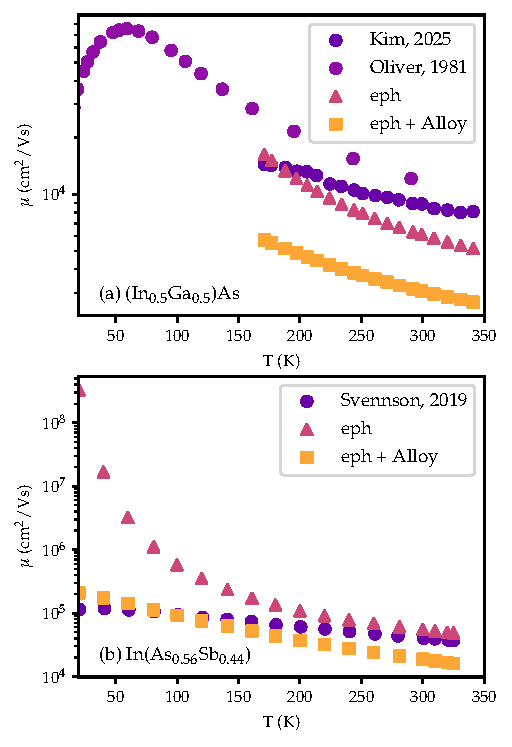
\includegraphics[width=\linewidth]{Figures/mobility_plot.1.pdf}
        \caption{Calculated electron mobility as a function of temperature for (a) (In$_{0.5}$Ga$_{0.5}$)As and (b) In(As$_{0.5625}$Sb$_{0.4375}$), showing the phonon-limited result and the result with alloy scattering included. Note the differing vertical scales: in (b) the phonon-limited mobility rises by four orders of magnitude as the polar optical modes freeze out below \SI{100}{\kelvin}, whereas the elastic alloy channel does not. Experimental data are from Kim \textit{et al.}\cite{Kim2025} for (In$_{0.53}$Ga$_{0.47}$)As and Svensson \textit{et al.}\cite{Svensson2019} for In(As$_{0.56}$Sb$_{0.44}$); the carrier concentrations reported in those works were used in the corresponding calculations.}
    \label{fig:mobility_plot1}
\end{figure}

The temperature dependence is shown in Fig.~\ref{fig:mobility_plot1}. The two channels behave quite differently. Polar optical scattering freezes out as the temperature falls, so the phonon-limited mobility of In(As$_{0.5625}$Sb$_{0.4375}$) rises by four orders of magnitude between \SI{300}{\kelvin} and \SI{25}{\kelvin}, far above any measured value. The alloy channel is elastic, and its rate varies with temperature only through the thermal distribution of carriers, so it falls away much more slowly and comes to dominate. With it included, the calculated mobility reproduces the measurements of Svensson \textit{et al.}\cite{Svensson2019} from \SI{25}{\kelvin} to roughly \SI{150}{\kelvin}. Since phonon scattering is negligible over that range, this is a direct test of the computed alloy potential, and the agreement supports both its magnitude and its temperature dependence.

Towards room temperature the mobilities of both alloys are underestimated by a factor of roughly $2.5$. This is the region in which polar optical scattering dominates, and therefore the region most sensitive to the Fr{\"o}hlich interaction, which Sec.~\ref{sec:eph_scattering} showed to be overestimated by \numrange{1.8}{3.0} in (InGa)As and \numrange{1.3}{1.7} in In(AsSb). The two alloys are affected differently. In In(As$_{0.5625}$Sb$_{0.4375}$) the phonon-limited mobility is high enough that the alloy channel is the only effective limit below \SI{150}{\kelvin}, where the agreement with experiment is good; the shortfall appears only as the polar modes become active towards room temperature. In (In$_{0.5}$Ga$_{0.5}$)As the phonon-limited result already falls below the measurements above \SI{200}{\kelvin}, before any alloy scattering is added, and the alloy channel only compounds this. Correcting the Fr{\"o}hlich coupling raises the phonon-limited mobility above the measured values, which indicates that the apparent agreement of the uncorrected result is fortuitous.

In the case of In(AsSb) the alloy scattering has been a previously significantly underestimated quantity, and is essential to understanding the total mobility.

\begin{figure}
    \centering
    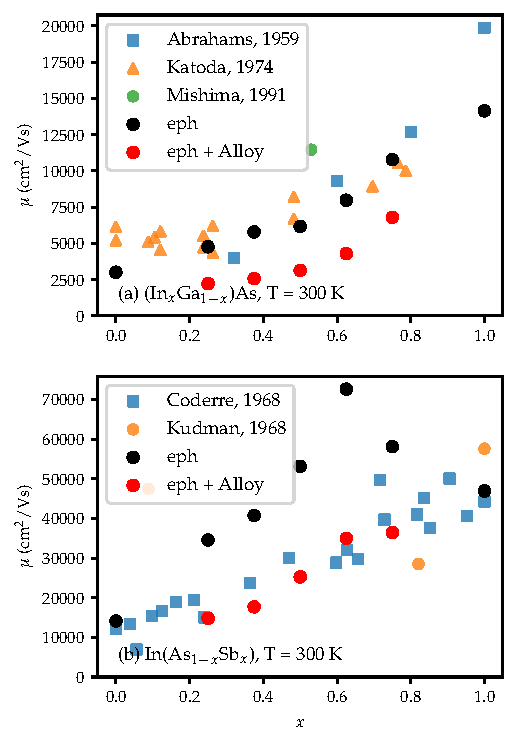
\includegraphics[width=\linewidth]{Figures/all_mobs_300K_offset.pdf}
    \caption{Calculated electron mobility at \SI{300}{\kelvin} as a function of composition for (a) (In$_{x}$Ga$_{1-x}$)As and (b) In(As$_{1-x}$Sb$_{x}$), with and without the alloy channel. A fixed carrier concentration of $n=\SI{1e16}{\per\cubic\centi\metre}$ was used throughout. Experimental values are those of Abrahams \textit{et al.}, Katoda \textit{et al.} and Mishima \textit{et al.} for (a), and Coderre \textit{et al.} and Kudman \textit{et al.} for (b), as compiled in Ref.~\onlinecite{Chattopadhyay1981}.}
    \label{fig:mobility_plot2}
\end{figure}

The variation with composition is shown in Fig.~\ref{fig:mobility_plot2}. For In(As$_{1-x}$Sb$_{x}$) the alloy channel substantially improves the agreement with the measurements of Coderre \textit{et al.}\cite{mob_Coderre1968}, and is clearly essential to describing transport in this alloy. The phonon-limited result alone varies far more sharply with composition than the data, peaking near $x=0.625$: both the effective mass and the band gap bow strongly in this system, and since $\epsilon_\infty$ rises as the gap narrows, the light mass and the weakened Fr{\"o}hlich coupling act together to raise the mobility at the same composition. Including alloy scattering flattens this variation, because the $x(1-x)$ factor in Eq.~\eqref{eq:alloy_rate} suppresses the mobility most strongly at mid-composition and vanishes at both binary endpoints.
For (In$_{x}$Ga$_{1-x}$)As the picture is different. The phonon-limited result already lies close to the measured values across the composition range, and adding the alloy channel takes it below them. Unlike Fig.~\ref{fig:mobility_plot1}, the carrier concentration here was not matched to the experiments, since the compiled data span a range of concentrations; we instead fix $n=\SI{1e16}{\per\cubic\centi\metre}$ throughout.
The conclusions drawn above about the Fr{\"o}hlich interaction apply equally to the composition dependence. The phonon-limited mobilities of (InGa)As only appear to agree with experiment: corrected for the overestimated coupling they lie well above it, and both they and the results including alloy scattering require readjustment. This cannot be done self-consistently within the present framework, but an estimate of the corrected values can be made.

Taken together, these results establish alloy scattering as a dominant mechanism in In(As$_{1-x}$Sb$_{x}$) and a substantial one in (In$_{x}$Ga$_{1-x}$)As. The computed potentials are an order of magnitude stronger in their effect on the scattering rate than the electronegativity estimates they replace, and in In(AsSb) they reproduce the measured low-temperature mobility without adjustment, in a regime where polar scattering is frozen out and the alloy channel acts alone. The agreement is less good in (InGa)As, where the alloy channel is evidently too strong: correcting $\epsilon_\infty$ to its converged value raises the calculated mobility by only a factor of $1.3$, which does not close the remaining discrepancy. Several of the approximations made in Sec.~\ref{sec:alloy_scattering} could contribute, of which the first Born treatment is perhaps the most likely: evaluating the matrix element between unperturbed virtual-crystal states neglects the relaxation of the scattering state away from the substituted site and so overestimates its overlap with $\Delta V$. Establishing this would require the supercell scattering states that the present approach is designed to avoid, and we leave it to future work.

\section{Conclusion}

We have presented a first-principles methodology for computing the electron mobility of direct-gap semiconductor alloys, and applied it to (In$_x$Ga$_{1-x}$)As and In(As$_{1-x}$Sb$_{x}$). The alloy is represented by a virtual crystal whose band structure is corrected by Hubbard $U$ parameters, fitted to the effective band structures of the supercell calculations of our previous work\cite{Gentles2026a} subject to the constraint that the effective mass reproduce its experimental value. The alloy scattering potential is then evaluated about $\Gamma$ by adapting the approach of Murphy-Armando and Fahy\cite{MurphyArmando2008}, and incorporated alongside the DFPT$+U$ electron--phonon elements in the iterative solution of the Boltzmann transport equation implemented in \texttt{PERTURBO}. This gives the phonon-limited and alloy-limited contributions to the mobility on an equal footing, within a single primitive-cell calculation.

The computed alloy coupling elements are three to four times larger than the electronegativity estimates they replace, corresponding to roughly an order of magnitude in the scattering rate. In In(As$_{1-x}$Sb$_{x}$) this larger coupling is required to reproduce the measured mobility: below \SI{150}{\kelvin}, where polar optical scattering has frozen out, the alloy channel alone accounts for the data without adjustment. The elements are moreover strongly dependent on $|\bm{k}|$ in both alloys, falling by \SIrange{20}{40}{\percent} across the transport window, which the constant square-well potentials of earlier treatments cannot represent. Their angular dependence is governed by which sublattice is alloyed: the $p$ admixture acquired by the conduction band away from $\Gamma$ is almost entirely anion-derived, so a perturbation on the anion sublattice couples to it and one on the cation sublattice does not. Earlier studies combined a constant potential with the relaxation time approximation and parabolic bands, none of which is adequate for alloys whose conduction bands are strongly non-parabolic within a few $k_\text{B}T$ of the band edge.

Two limitations bear on the quantitative agreement. The dielectric constants obtained from the VCA$+U$ band structure are systematically too small, which strengthens the Fr{\"o}hlich coupling and depresses the mobility wherever polar scattering dominates; we find the mobility to be as sensitive to $\epsilon_\infty$ as it is to the effective mass, so that constraining both would require a further condition on $\bm{U}$. The alloy matrix elements are evaluated in the first Born approximation between unperturbed virtual-crystal states, which neglects the relaxation of the scattering state about the substituted site. The latter is the more likely source of the residual overestimate of alloy scattering in (In$_x$Ga$_{1-x}$)As.

The method requires no fitted scattering parameters, and reduces the cost of an alloy transport calculation to that of a primitive cell. It should extend directly to the remaining III--V ternaries and, with a second mixed sublattice, to quaternaries such as (In$_x$Ga$_{1-x}$)(As$_{1-y}$Sb$_y$), for which no first-principles alloy scattering potentials exist.

\section{Computational Details}\label{sec:details}

All DFT calculations were performed using \texttt{Quantum ESPRESSO}\cite{QE1,QE2,QE3} with the Perdew-Burke-Ernzerhof\cite{Perdew1996} GGA functional, with the Hubbard correction calculated within the Dudarev formulation\cite{DFTU_Dudarev} on the valence $p$ orbitals. The pseudopotentials were norm-conserving scalar relativistic from Pseudodojo version 0.5\cite{pseudodojo1,pseudodojo2}. 
The kinetic energy cutoff used was $E^\text{wfc}_\text{cutoff}=$\SI{120}{\rydberg}, with the electron density cutoff set as $E^\rho_\text{cutoff}=4E^\text{wfc}_\text{cutoff}$, which is the default value. The k-point meshes varied depending on the type of calculation. With the primitive cells, relaxation calculations used $12 \times 12 \times 12$ grids, while the SCF calculations and NSCF calculations used $16 \times 16 \times 16$ grids, along with the wannierization. The DFPT+U calculatiosn used $8 \times 8 \times 8$ q-point meshes. The 64-atom $2 \times 2 \times 2$ atom supercells calculated for the phonon densities of states used $2\times 2 \times 2$ calculations, which are sufficient for the forces to converge. The 216-atom $3 \times 3 \times 3$ supercells used for the alloy scattering calculations used $\Gamma$-point calculations k-point meshes for the cell relaxation, and $2 \times 2 \times 2$ meshes for the SCF calculations. The potentials were transferred to real space on the default grids without interpolation, $240 \times 240 \times 240$ for (InGa)As and $270 \times 270 \times 270$ for In(AsSb). Our own code was used to generate the fourier transform of the primitive cell wavefunctions to real space, as well as calculating the alloy scattering elements. 
The Hubbard parameters $\bm{U}=(U_A,U_B)$ obtained for each composition, together with the extrapolated dielectric constants and their fitted exponents, are tabulated in the Supplemental Material.

The wannierization was performed using \texttt{Wannier90}\cite{w901_Mostofi2008,w903_Pizzi2020} with the self-consistent density matrix initial estimates, and the \texttt{erfc} disentanglement procedure for 4 valence and 4 conduction bands, where teh frozen window sits below the bottom of the 5\textsuperscript{th} conduction band, and the maximum just above the top of the 4\textsuperscript{th} band maximum, and the electron-phonon coupling elements were calculated using \texttt{Perturbo}\cite{Perturbo1}. The mobilities were calculated using the ITA as implemented in \texttt{Perturbo}, with the alloy scattering added to the code. The alloy scattering was also implemented with in the \texttt{Perturbo} code framework. 

All of our code and calculations are available in our Zenodo repository[CITE our data].

\section*{Acknowledgments}

The research leading to these results has received funding from the Austrian Research Promotion Agency FFG (project n895289). The computational results have been achieved using the ARCHER2 UK National Supercomputing Service (https://www.archer2.ac.uk) for the supercell calculations, and the Austrian Scientific Cluster (https://asc.ac.at/systems/vsc-5/) for the optimization calculations. Thanks are also given to Anna Benzer, Martin Loesener, and Gerald Wisb{\"o}ck for formational discussions and technical expertise.

\nocite{}
\bibliographystyle{apsrev4-2}
\bibliography{refs}

\end{document}
